% Appendix (not counted towards the word limit).
\clearpage
\section{Example prediction}
\label{app:example}

The output below is what Assignment~3's back end receives. It was produced by
\code{python -m explorer.cli predict what-if} on a hypothetical transaction of one DS1 address: sending
0.05~BTC, about a hundred times the address's usual amount. The size features (F1, F4) pass the flag line;
the timing features (F2, F3) are within the usual range, so they are not mentioned.

{\footnotesize
\begin{verbatim}
input:    0.05 BTC out at 2026-10-20T12:00Z, address 1Bbcsfxj2JRUD5crcdZVHBcViT61vrJ3dz
scored: true   flagged: true   score (largest |z|): 5.98
feature                     value        usual       z  role
F1 Size                      0.05  0.000524948    5.88  flag
F2 Burst                        3            4   -0.45  within-usual
F3 Gap                    21.8264      10.0535    0.30  within-usual
F4 Relative size          95.2472     0.909938    5.98  flag
\end{verbatim}
}
Explanation shown to the user (template writer):
{\footnotesize
\begin{verbatim}
Flagged by Robust z baseline (A1).
What stands out compared with this address's own history:
- Higher ratio to the usual amount than usual: 95.2x the usual amount for this direction, against a
  usual 0.9x.
- Larger amount than usual: 0.05 BTC moved, against a usual 0.00052495 BTC.
Unusual activity requires investigation; it does not indicate wrongdoing.
\end{verbatim}
}


\section{Further results}
\label{app:figures}

\begin{figure}[H]
\centering
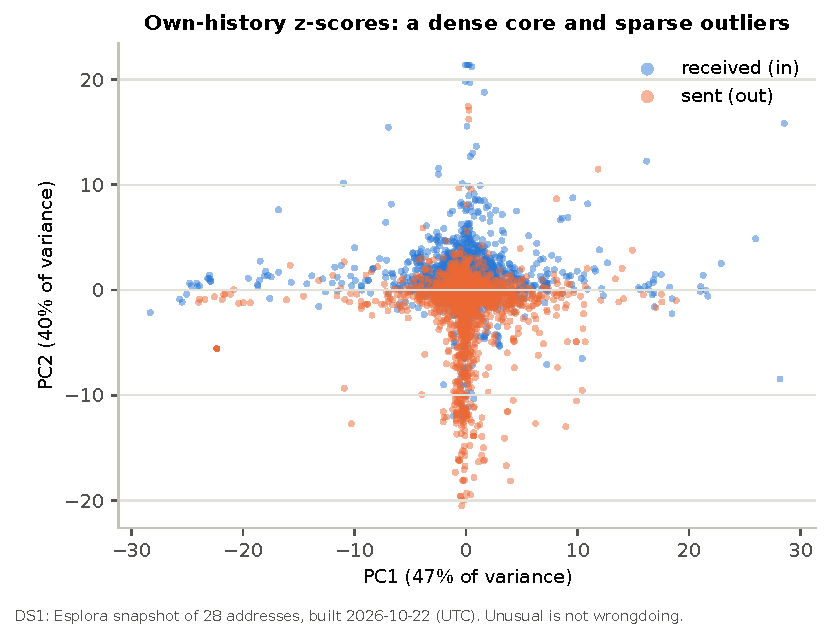
\includegraphics[width=0.78\textwidth]{eda_pca.pdf}
\caption{DS1's transactions on the first two principal components, showing a dense core with sparse outliers
(Finding~3).}
\label{fig:pca}
\end{figure}

\begin{figure}[H]
\centering
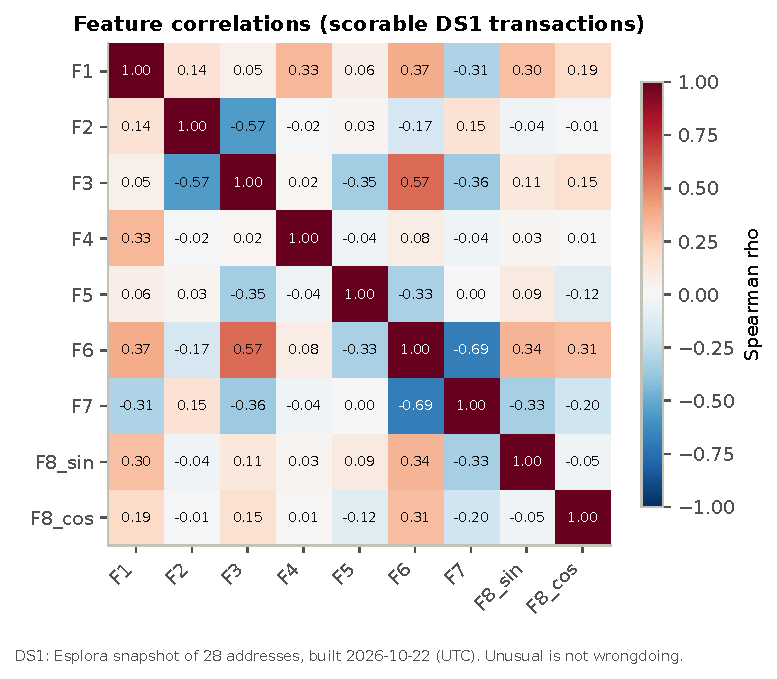
\includegraphics[width=0.72\textwidth]{eda_feature_correlation.pdf}
\caption{Rank correlations between DS1's features (Finding~3).}
\label{fig:correlation}
\end{figure}

\begin{figure}[H]
\centering
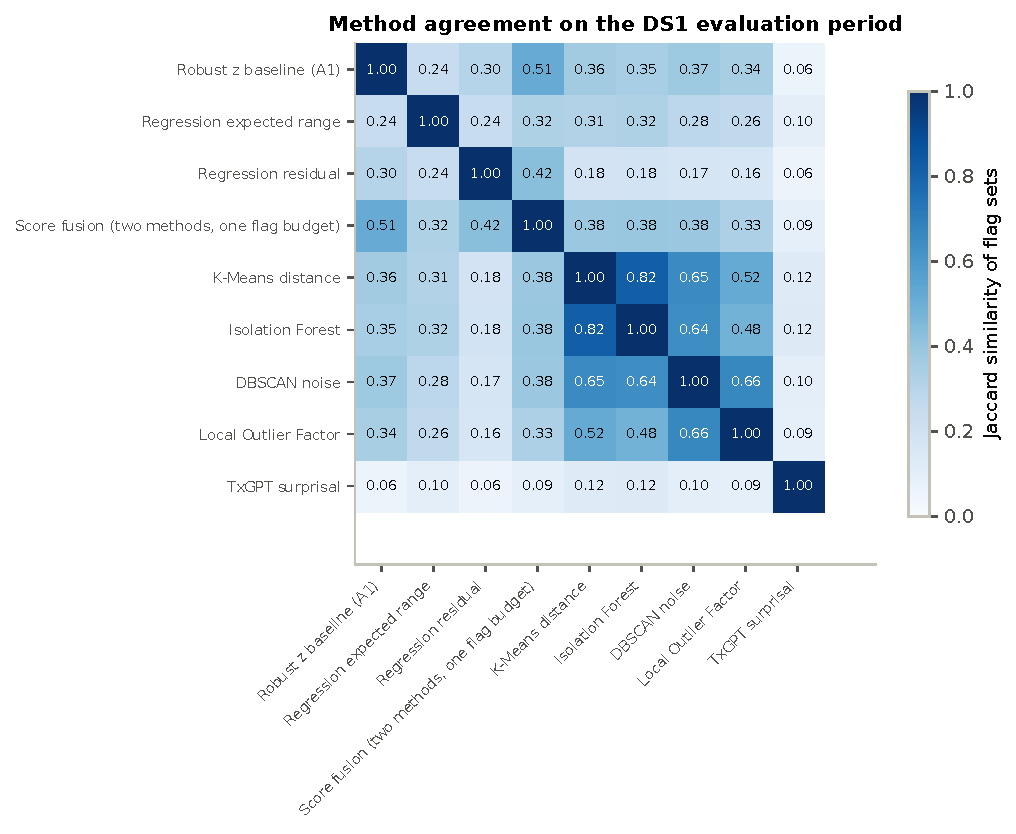
\includegraphics[width=0.78\textwidth]{eval_agreement.pdf}
\caption{Pairwise Jaccard overlap between the methods' flagged transactions (\code{eval\_agreement.csv}).}
\label{fig:agreement}
\end{figure}

\begin{figure}[H]
\centering
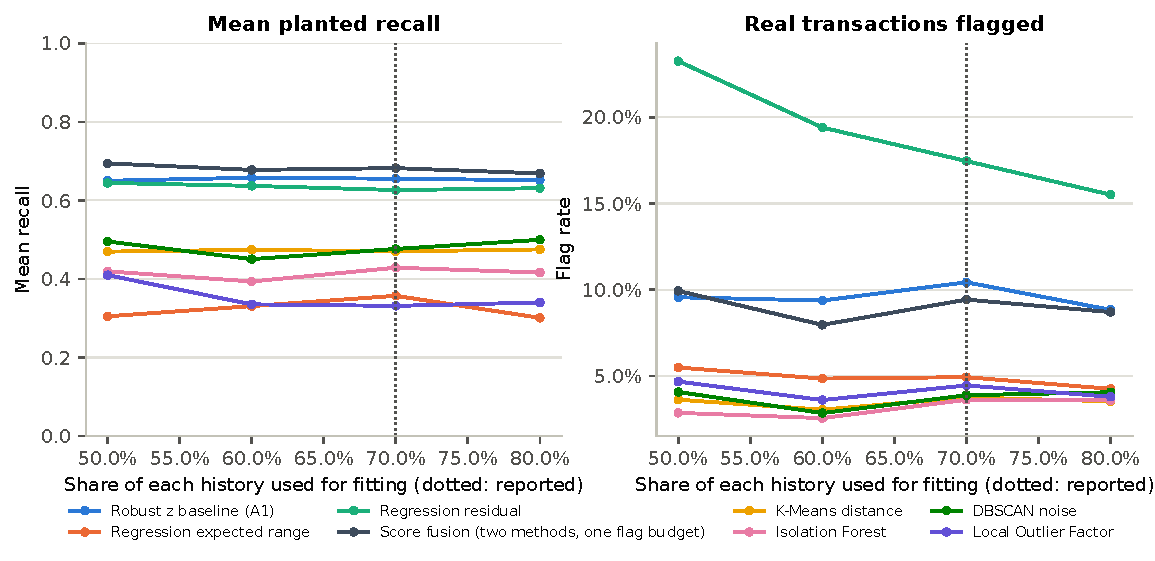
\includegraphics[width=0.85\textwidth]{eval_walkforward.pdf}
\caption{Every method refitted at each walk-forward cut-off (\code{eval\_walkforward.csv}).}
\label{fig:walkforward}
\end{figure}

\begin{figure}[H]
\centering
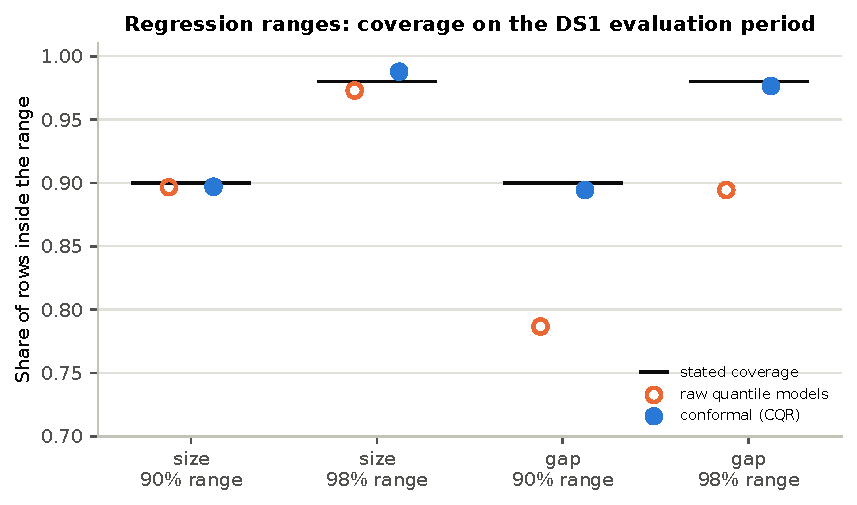
\includegraphics[width=0.8\textwidth]{eval_conformal.pdf}
\caption{Coverage of the regression ranges before and after conformal calibration
(\code{regression\_results.csv}).}
\label{fig:conformal}
\end{figure}

\begin{figure}[H]
\centering
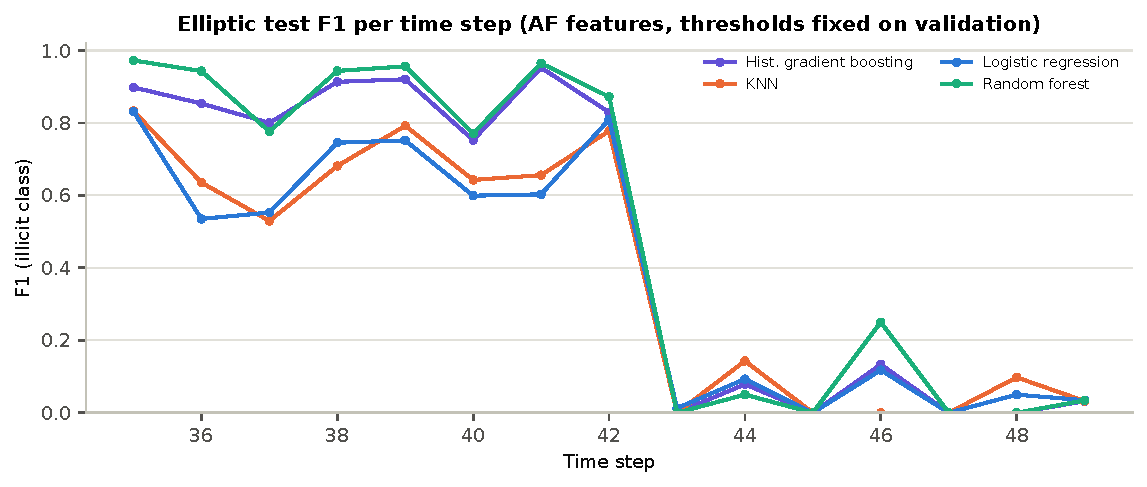
\includegraphics[width=0.82\textwidth]{eval_elliptic_f1_by_step.pdf}
\caption{Elliptic test F1 per time step. Every model fails from step 43, after the shutdown of a dark market
changed the illicit class's behaviour.}
\label{fig:elliptic}
\end{figure}

\begin{figure}[H]
\centering
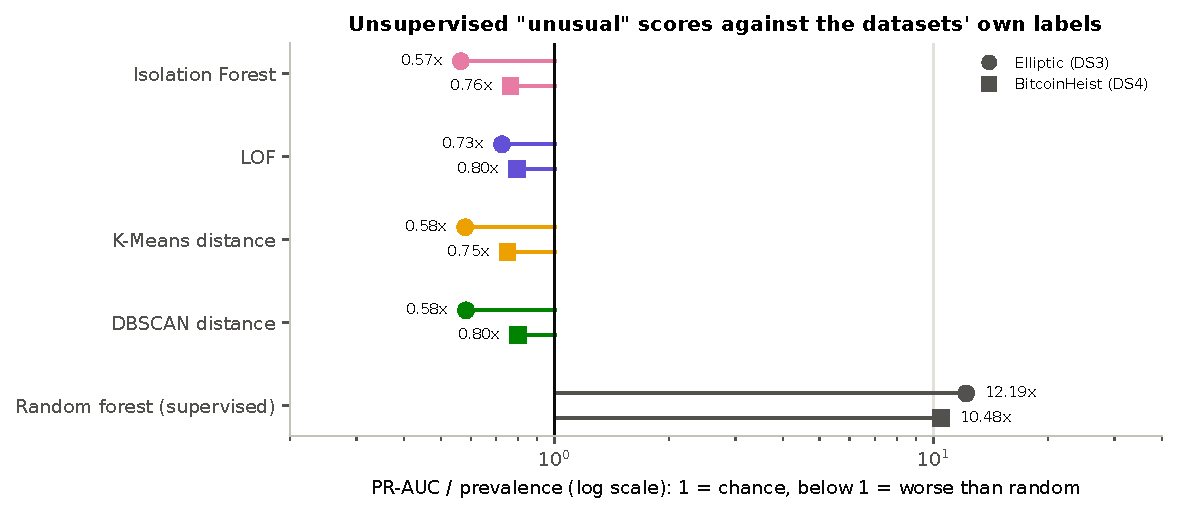
\includegraphics[width=0.9\textwidth]{eval_label_check.pdf}
\caption{Unsupervised scores against the labelled datasets' own classes. Every unsupervised method is below
chance (1$\times$), while the supervised random forest is far above it: being unusual is not the same as
belonging to a labelled class (\code{label\_check.csv}).}
\label{fig:labelcheck}
\end{figure}

\begin{figure}[H]
\centering
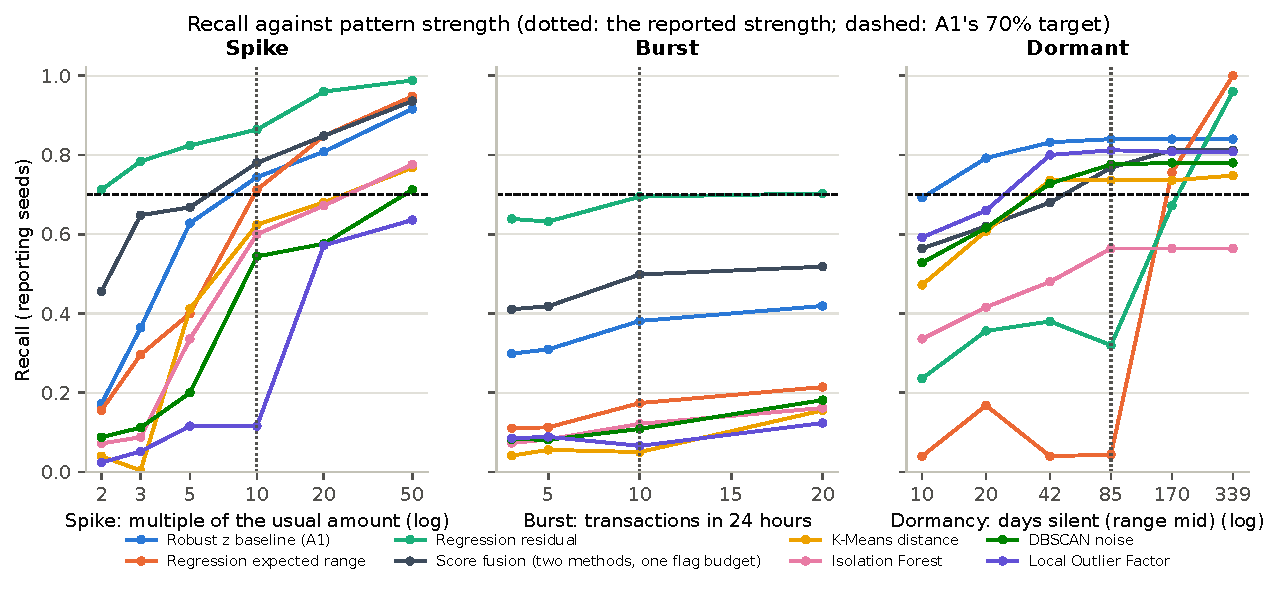
\includegraphics[width=0.9\textwidth]{eval_sensitivity.pdf}
\caption{Recall against the strength of each planted pattern (\code{eval\_sensitivity.csv}). Weaker plants are
harder for every method; regression keeps finding small spikes that the baseline misses.}
\label{fig:sensitivity}
\end{figure}

\begin{figure}[H]
\centering
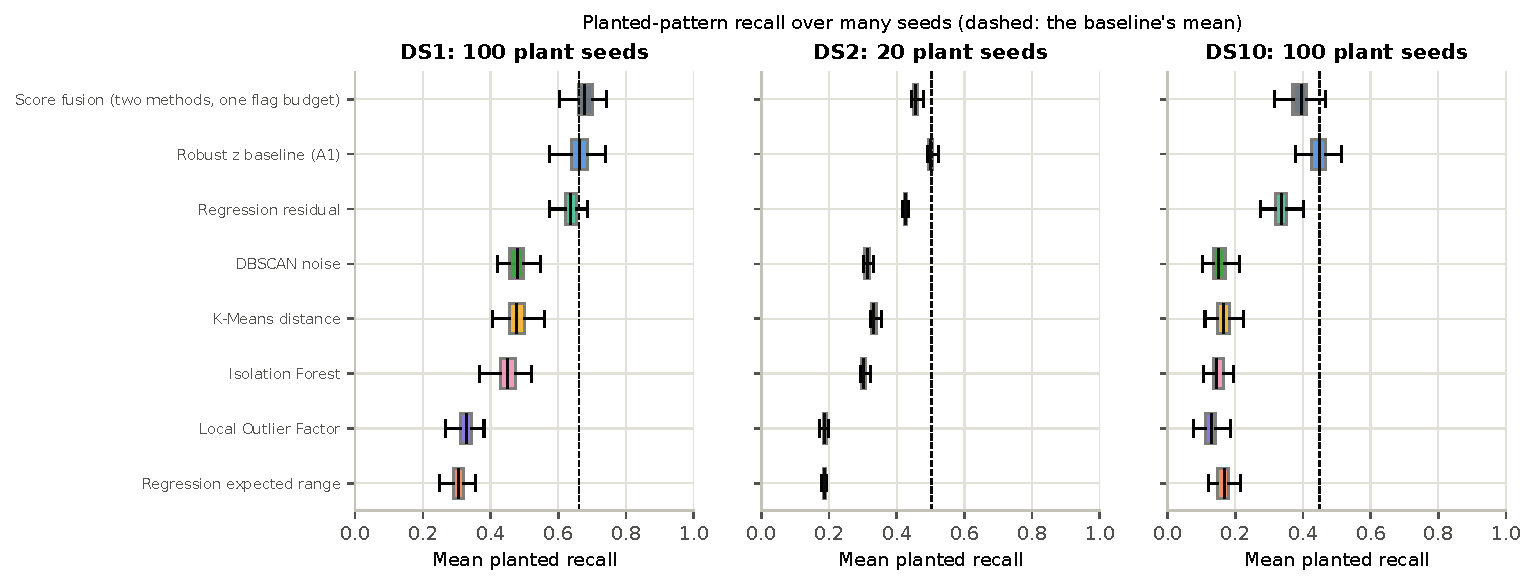
\includegraphics[width=0.9\textwidth]{stats_methods.pdf}
\caption{Mean planted recall over 100 plant seeds on DS1 and DS10 and 20 on DS2
(\code{stats\_methods\_summary.csv}).}
\label{fig:statsmethods}
\end{figure}

\begin{figure}[H]
\centering
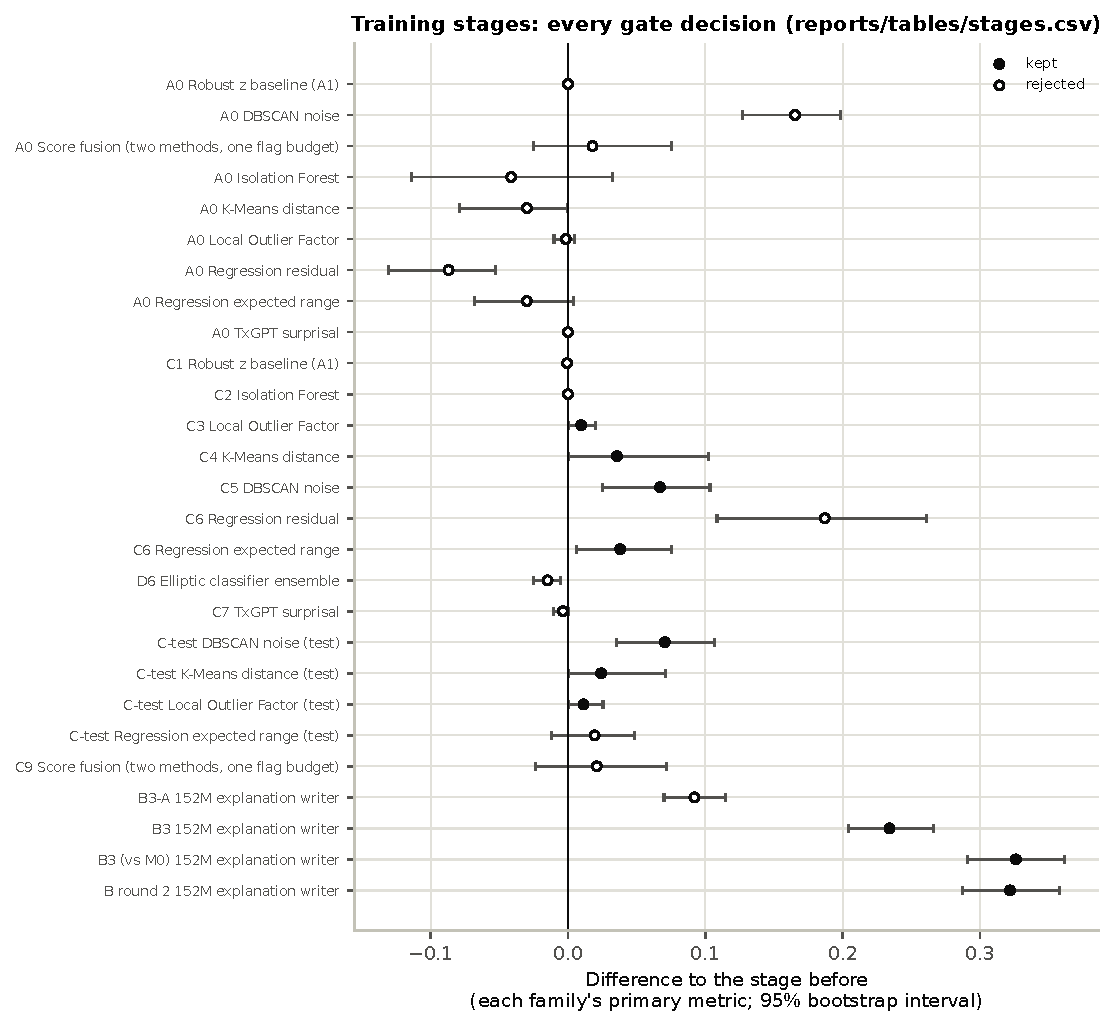
\includegraphics[width=0.9\textwidth]{eval_stages.pdf}
\caption{Every training stage's gate decision with its bootstrap interval (\code{stages.csv}).}
\label{fig:stages}
\end{figure}

\begin{figure}[H]
\centering
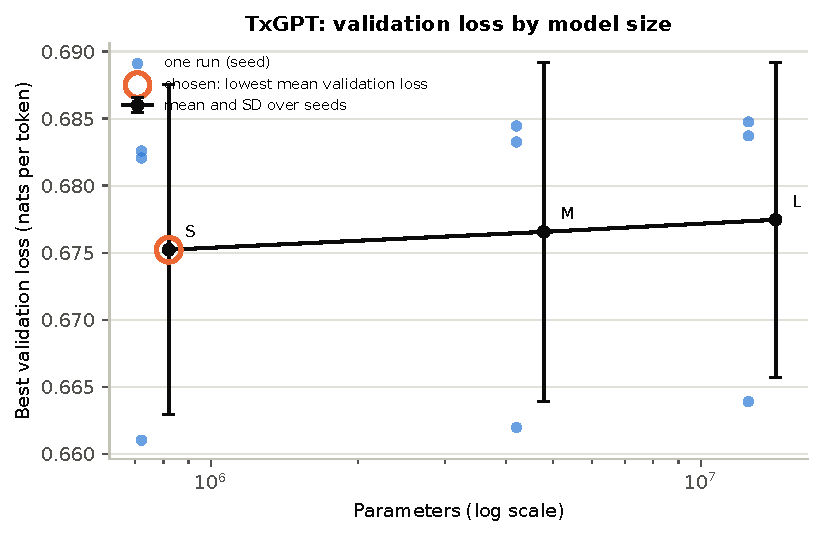
\includegraphics[width=0.75\textwidth]{eval_txgpt_sizes.pdf}
\caption{TxGPT's validation loss for three sizes and three seeds each (\code{txgpt\_sizes.csv}). The sizes tie,
so the smallest was kept.}
\label{fig:txgpt}
\end{figure}

\begin{figure}[H]
\centering
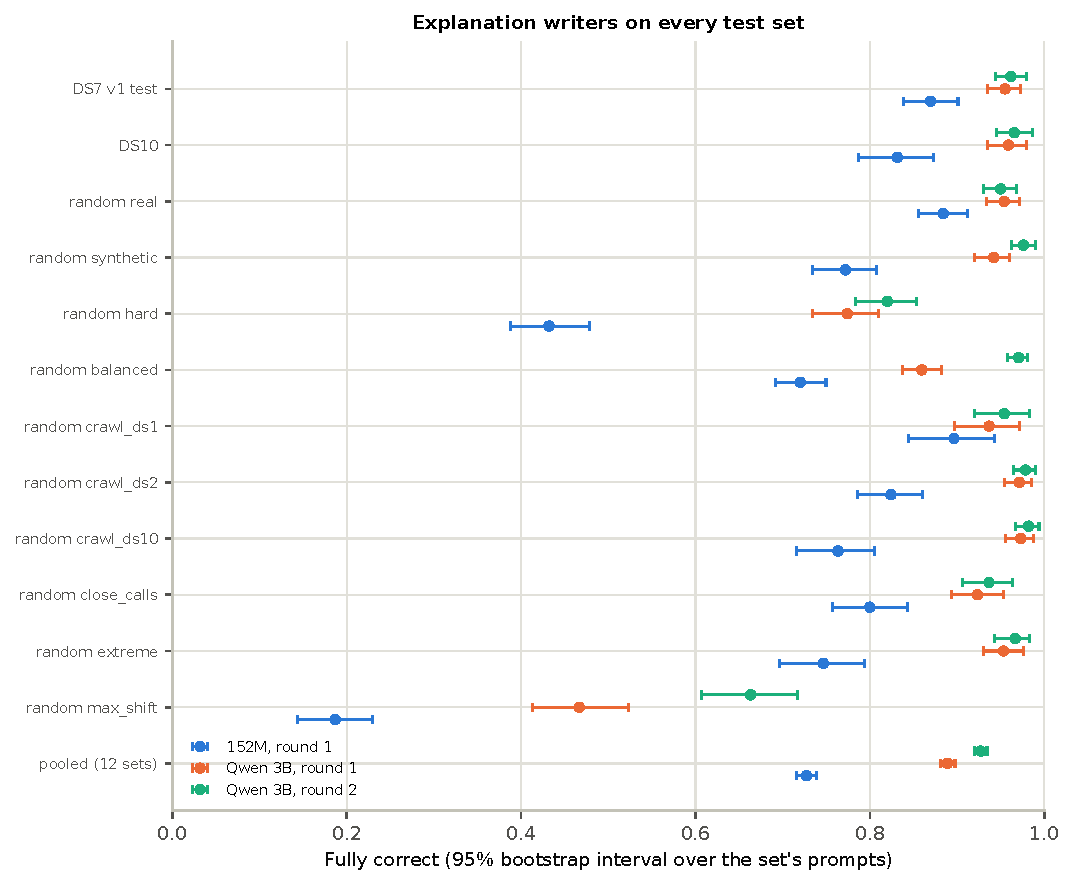
\includegraphics[width=0.9\textwidth]{stats_writers.pdf}
\caption{The Assistant's fully correct rate on each test set, before (round 1) and after (round 2) its second
training round, with 95\% bootstrap intervals (\code{stats\_writers\_summary.csv}).}
\label{fig:writers}
\end{figure}

\section{Reproducing the results}
\label{app:repro}

The repository's \code{README.md} gives every command. In short:
\begin{verbatim}
conda env create -f environment.yml
conda activate cos30049-a2
python -m pytest -q                     # the test suite
python -m explorer.cli all --offline    # every DS1 result
python -m explorer.cli figures
python tools/compare_tables.py          # rebuild against the committed tables
\end{verbatim}
\code{DATA\_CARD.md} documents every dataset, file and column, and \code{MODEL\_CARD.md} every final model.
